\documentclass{article}
%%%%%%%%%%%%%%%%%
%%% Preambles %%%
%%%%%%%%%%%%%%%%%

\usepackage[margin=1in, includefoot]{geometry}
\usepackage{url}

%% References
\usepackage[backend=biber,style=authoryear, sorting=nyvt, maxcitenames=3]{biblatex}
\addbibresource{References.bib}
\usepackage[utf8]{inputenc}

% Images
\usepackage{graphicx}  % Allows importing images.
\usepackage{float}     % Allows for control of float positions.



% Tables
\usepackage{caption} 
\captionsetup[table]{skip=10pt}
\usepackage{array}
\newcolumntype{@}{>{\global\let\currentrowstyle\relax}}
\newcolumntype{^}{>{\currentrowstyle}}
\newcommand{\rowstyle}[1]{\gdef\currentrowstyle{#1} #1\ignorespaces}
\usepackage{booktabs}
\usepackage[flushleft]{threeparttable}



% Header and Footer
\usepackage{fancyhdr}
\pagestyle{fancy}
\fancyhead{}
\fancyfoot{}
\fancyfoot[R]{\thepage}
\renewcommand{\headrulewidth}{0pt}
\renewcommand{\footrulewidth}{0.5pt}


\begin{document}

%%%%%%%%%%%%%%%%%%%%%%
%%%% Front matter %%%%
%%%%%%%%%%%%%%%%%%%%%%

%% titlepage
\thispagestyle{empty}
\begin{titlepage}   % Frontpage
	\begin{center}      % Titlepage Titles
		\line(1,0){350}\\
		\huge{\bfseries Forest Induced Convection}\\
		[-4mm]
		\line(1,0){350}	\\
		[0.75cm]
		\textsc{\Large Cloud analysis using satellite images}\\
		[1.5cm]
		\textsc{\LARGE MSc Thesis Proposal}\\
		[1cm]
		\textsc{\large R.C. Maas\\
		February, 2016 \\
		[10cm]}
	\end{center}
	\begin{flushleft}   % Titlepage Info
		\textsc{\large Rob Maas\\
			e-mail: rob.maas@wur.nl \\
			HWM group \\
			Wageningen UR\\
			StudentID: 890712537130 \\}
	\end{flushleft}
\end{titlepage}


%% Table of contents
\tableofcontents
\thispagestyle{empty}
\cleardoublepage

%%%%%%%%%%%%%%%%%%%
%%%% Main Body %%%%
%%%%%%%%%%%%%%%%%%%
\pagenumbering{arabic}
\setcounter{page}{1}

\section{Introduction}\label{sec:intro}   % Introduction
\subsection{Background}
Clouds are important for regulating the weather and climate, locally and globally \parencite{tiedtke93}. Locally the clouds are responsible for precipitation and thunderstorm events, and through their high reflectivity they influence the global energy balance substantially  \parencite{hartmann92}. The low altitude clouds inside the boundary layer, e.g. cumulus clouds, are a crucial part in the hydrologic cycle as they control the upward transport of moisture \parencite{arellano12}. Studies show that changes in this hydrologic cycle do affect the climate \parencite{pielke98}, and vice versa. In another study it is confirmed that the ongoing climate change has a large effect on cloud cover \parencite{arellano12}. Understanding the mechanisms behind cloud formation is therefore crucial to create reliable weather and climate models.\\

Many meteorological studies have investigated relations between atmospheric variables and cloud formation, and the impact of climate change on clouds. However, the impact of forests on clouds is a subject that has hardly been studied. Many hydrological characteristics are different for forests than for other land uses, resulting in typical responses from forests to for example heatwaves \parencite{teuling10}. Therefore it is to be expected that the forests will have a different effect on the formation of clouds. To correctly implement forests into the weather models, it is essential to study these effects. Furthermore, the ongoing global intensification of agriculture is causing a vast decrease of natural ecosystems, including forests. On the other hand, active forest management is improving forest conditions, protecting ecosystems and creating new forests elsewhere, increasing the standing biomass of European forests by about 40\% \parencite{foley05}. To simulate and study the effect of the ongoing and future forest adaptations on regional and global scale it is necessary to further understand the dynamic relation between forests and clouds.\\

Most studies so far that relate to this topic have been conducted in the Amazon \parencite{chagnon04}, and while this area benefits from almost no human influences, it is not very practical for weather forecasting. Areas that would benefit most from improvements in the models are areas with a dense population, therefore I choose to study the effect of West European forests. Where most previous studies relied on observation from the ground,  I will use satellite data for the cloud observations. From a preliminary study of this data it is already evident that also in Europe there is more cloud formation above forests than above neighbouring grasslands under certain circumstances (Figure \ref{fig:cloudsoverforest}). To get a further understanding of this phenomenon, I will process and study the large amount of satellite images that are available to find out under which conditions the clouds form and what they contribute to the total cloud budget.

%Figure cloudsoverforest
\begin{figure}[H]
	\centering
	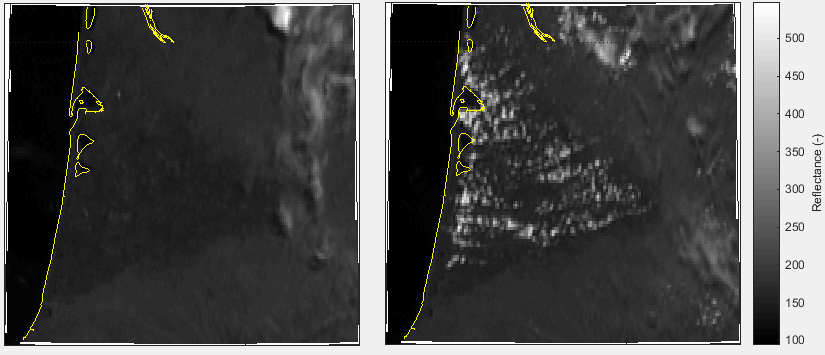
\includegraphics[height=3in]{figures/cloudform1.png}
	\caption{Satellite images of the Landes area in South west France, taken two hours apart. Left) Only some inland clouds visible, but the coastal area is completely cloudless. Right) Clear cloud formation above the Landes forest, only two hours after the sky was clear. }
	\label{fig:cloudsoverforest}
\end{figure}

Reasons for the different behaviour of clouds above forests were given in previous meteorological studies. They show that deforested areas in rainforests affect the type and density of the cloud cover. Shallow clouds are forming over the deforested areas, while there are only deep clouds over the dense forest \parencite{chagnon04}. The difference in length scales \parencite{irvine97} and temperature between the deforested and forested areas cause convective mesoscale circulations \parencite{souza00}, which act as a lifting mechanism for the shallow clouds above at the transition zones. The difference in length scale and temperature between the forest and arable farmland will likely play a role in Western Europe as well. However, the additional cloud formation is not always visible, so there must be an additional factor that is probably accounted for by the weather conditions. The synoptic weather largely controls the air humidity and air temperature, which are important for cloud formations. So an important part of understanding the relation between forests and clouds is to find out which weather variables (e.g. wind speed, direction, temperature) are important.\\

Although the results from the research in the Amazon cannot directly be applied to European situations, it is evident from the research that mesoscale circulations only occur if the difference in length scales is high enough and the temperature difference is large enough. Only then there will be enough heterogeneity to trigger the circulations. Also enough Convective Available Potential Energy (CAPE) and moisture is needed for the circulations to develop into deep convective clouds. These properties are all related to the size of the forest, and it is therefore likely that the forest size is also a determining factor in the dynamics of cloud development. If a forest is too small, it is unlikely that there is enough CAPE and moist available for a convective cloud to develop. Knowing the minimum size of a forest before it starts to develop clouds is essential for correct implementation of the results in for example weather forecast models.\\

The images of Figure \ref{fig:cloudsoverforest} are showing the typical convective clouds over a French forest, but it is important to know how often the circumstances are right for these clouds to form. Only if we compare the forest induced clouds with the total cloud budget, some of the implications become clear and we can find out how relevant the clouds are in a bigger picture. Also other consequences of the additional clouds can be looked at, for example its effect on the albedo. Typically a forest has a lower albedo than other land uses, but if there are significantly more clouds above forests, this might (partially) make up for the lower albedo of the trees.

A critical part of this research in the planetary albedo map that contains the surface reflectance for each pixel under cloudless conditions, depending on the time and the day of the year. The images are compared with this map, and if the reflectance value is significantly higher (based on a threshold, see Approach section) the pixel is flagged as a cloud. I choose to create this map based on the satellite data, to make sure it is very compatible and that it can safely be compared with the satellite images, without any conversion. Creating the map myself also ensured that there is different reflectance data available for every image, depending on the time and date it was taken. But it is necessary to investigate how well this background albedo map performs, before we can use it for the rest of the study.

\subsection{Objectives}
The problems described in the previous section are to be addressed in this research. To analyze under which conditions additional cloud formation occurs above forests and how relevant this is, this study aims to answer the following research questions. \\

For forests in Western Europe I aim to find out:
\begin{enumerate}
	\item How well does the created albedo map perform?
	\item Which synoptic weather variables are the most important for cloud formation?
	\item Is there a minimal forestsize required for cloud formation to occur?
	\item What implications do the forest induced clouds have for the total cloud budget and the albedo?
\end{enumerate}


%% Material and Methods
\newpage
\section{Material and Methods}  % Material and Methods
In this section I will first describe the area that was chosen for the research. I will then describe the data in more detail. After which the approach for tackling each of the research questions will be described. Followed by a short estimation of our feasibility of completing the research successful, an overview of the materials and software needed and finally a short overview of the planning.

\subsection{Study Areas}
For this study the area that will be investigated has to fulfil a number of requirements to make it useful for every objective. First of all the area has to be located in Western Europe. Secondly, the conditions for the forests and the surrounding areas should be as equal as possible to minimize influences from other sources. Therefore the area needs to be relatively flat to reduce orographic effects, especially in the direction of the dominating wind direction. Furthermore, the area must contain different forest sizes, ranging from small to as large as possible.\\

With these conditions we chose the Western part of France to be our study  \ref{fig:studyarea}. We will specifically look more closely to two large forests, namely the Landes forest underneath Bordeaux and the Sologne forest near Orleans. The forests are situated in the Aquitaine and Paris Basin, that subsided in the Triassic and have been filled with a thick layer of sediments from the Pyrenean and Massif Central mountain ranges. The sedimentary basin resulted in a relatively low relief in the whole area, reducing orographic effects to a minimum. The dominating wind direction in the area is from the West and South-West, straight from the Atlantic Ocean, this results in parallel winds and equal weather circumstances for the entire area.

% Figure Study Area
\begin{figure}[H]
	\centering
	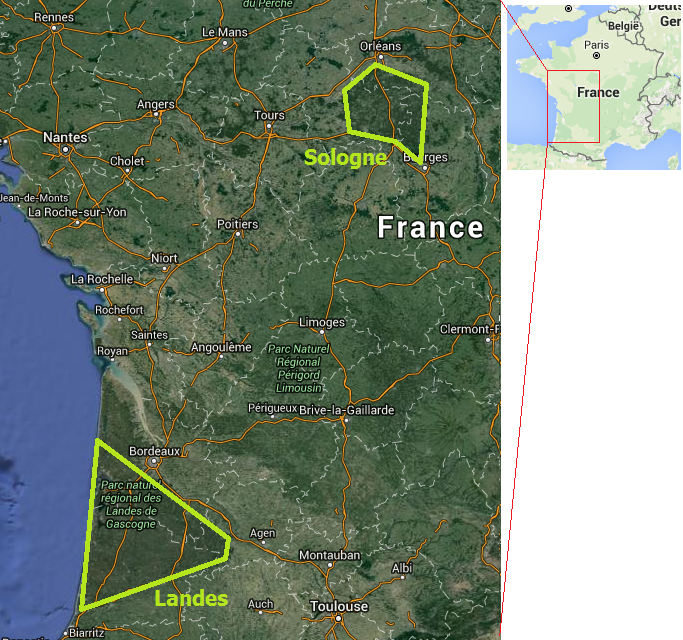
\includegraphics[height=4in]{figures/Study_area.png}
	\caption[Optional caption]{Southwestern part of France, with the Sologne and Landes forests highlighted, which will be the main study areas of this research. Images were taken from Google Earth.}
	\label{fig:studyarea}
\end{figure}


\subsection{Satellite data}
For the study I will at least use satellite data from two sources, the Meteosat second generation satellite and a weather product developed by the royal Dutch meteorological institute; MSG CPP. In this section a short overview is presented of the two data sources and some of their properties.

\subsubsection{Meteosat Second Generation}
For this research we will have satellite data available for the summer months (May,June, July and August) of the years 2004-2013, with a temporal resolution of one image every 15 minutes between 6 am and 6 pm. These images are products from the Meteosat Second Generation (MSG) satellite, which is a geostationary satellite designed by the EUMETSAT to monitor weather and climate from space \parencite[see][]{msg}. The MSG satellite carries a Spinning Enhanced Visible and Infrared Imager (SEVIRI) instrument that monitors twelve channels, each with different characteristics and applications (Appendix A). The data is available as level 1.5 data, which means that it has been pre-processed to undergo radiometric and geometric corrections. An example of these corrections are removal of disturbance caused by different atmospheric conditions, solar angles or temperatures between each image. The temporal resolution of the MSG is an image every 15 minutes.\\

Channel 12 will be the most useful for this study, as the spatial resolution of this channel is three times higher than then other channels. The bandwidth of this channel has been broadened to ensure enough incoming spectral radiance for sharp images; 400 – 1100 nm. A bandwidth this broad can mainly be used to distinguish clouds and a few land use types, but it is too small to differentiate between certain types of forest for example. But for this research, the broadband is sufficient and will net a resolution of 1x1km pixels.

\subsubsection{MSG Cloud Physical Properties}
The royal Dutch meteorological institute (KNMI) has developed an algorithm that uses the level 1.5 MSG data to deduct many other cloud properties, the so-called MSG Cloud Physical Properties-algorithm (MSGCPP) \parencite[see][]{msgcpp}. A full list of all the properties that the MSGCPP provides is available in Appendix A. The level 2 CPP products are freely available through their web viewer, but for this research we downloaded the relevant data so we can process them further ourselves. Although the CPP algorithm provides us with much additional information about the clouds, they are based on channels 1 through 11 of the MSG which means that the CPP products have a pixel size of 3x3km. Therefore this data will mainly be used for explanatory purposes.\\

The algorithm works in three steps, first it separates the cloud filled and cloud free pixels. Then the reflectances in the visible (0.6 $\mu m$) and near-infrared (1.6 $\mu m$) parts of the spectrum of the cloud filled pixels are compared with values in a database. The database (a look-up-table, LUT) contains the values of the primary cloud properties for every combination of reflectances. These values have been calculated using a radiative transfer model. Another set of secondary properties are then derived from the primary cloud properties.

\subsection{Approach}
In this section the approach to investigating each of the four research questions is presented. As this proposal is written at the start of the research, not many details are known yet about how everything is going to be done. However, we do present the ideas we have so far, and for the final report this section will be replaced by the actual methods, including the necessary details.

\subsubsection{Comparing the albedo map}
To investigate how well the albedo map that was created performs, it will be compared with high resolution albedo maps from other sources, such as the MODIS albedo product. Doing so will tell us if the relative difference between the forest and grassland areas is realistic and reliable.


\subsubsection{Identifying important weather variables}
For identifying which synoptic weather variables are playing a role for the development of additional clouds I only consider spring and summer months. Winter months are much more defined by large depressions and frontal weather systems that cover large areas with thick clouds, making it unable to distinguish additional clouds above forests. The summer months are much more stable and much more energy is available for convection.\\

The large Orleans and Landes forests will be compared with neighbouring grassland areas. Analysis will be done using scripts that will first determine for each image which pixels are filled with clouds, and which are not. The script will then compare for each image the forest with the non-forest areas to identify when there is significantly more clouds above the forests. When this is determined, the timestamps are statistically cross-referenced with a few synoptic variables that are likely to cause the additional convection, such as wind direction, wind speed, temperature and perhaps air moisture, as well as any combination of variables, using non-linear regression. These variables will be based on literature research. From the results we expect to see which variables are the most dominant factor for the additional cloud formation.

\subsubsection{Investigating importance of forest size}
After identifying which synoptic weather variables are important for additional cloud formation over the large forests, I select timeframes in which these are present. This means that we have a subset with additional clouds forming over at least the large forest, and the days with frontal weather situations are filtered out. Smaller regions are then selected and the cloud detection script will be used again to see if there are still significantly more clouds above the smaller forests than above the control regions. And if this is the case, if the difference is as large as with the larger forest or that there perhaps is another relation.

\subsubsection{Implications of additionally formed clouds}
When I know how often the weather is favouring additional cloud formation, from the timestamps found in the first research question. And when it is known for which forest sizes these mechanics play a role, we can assess for how much percentage of time this effect occurs for which percentage of the land surface. From that I can conclude how relevant these mechanics are for larger and smaller scales. For a local and regional scale the effects are likely to be larger than for the entire country, because relatively there are more forests in our study regions on a national scale. So this assessment will be made for a few spatial scales; local, regional and national. On a continental scale an assessment can perhaps be made by comparing the Landes and Sologne forests with larger forests to see if they are of the same type and in the same climatic zone, to see if these additional clouds are to be expected in larger areas as well.\\

Furthermore, the results can also temporally be extrapolated by looking at the relevant weather variables, and the development of these variables according to climate change scenarios. For example, if the cloud convection is positively correlated with temperature, there will likely be more additional cloud formation above forests in the future due to global warming. Based on literature and the outcomes of the other research questions something can be said about the impact of these mechanics, and whether they should therefore be implemented into weather and climate models.\\

The implications of the additionally formed clouds on the albedo of the forest can be determined by simply averaging the surface reflectance of each pixels of the raw data, to see if these values are relatively closer together than the pure albedo's that are determined using cloud-free pictures.\\

\subsection{Materials and Software}
As this study is purely an analytical study without field work, the only real piece of material that is required is a computer. I've been granted a computer workstation in the thesis room, which I will regularly use for the bulk of my research. When I get to the point where large quantities of data needs processing I can choose to run the scripts on my Linux-laptop, so I can continue working on my desktop computer.\\

A lot of raw data is needed to do the analysis of this research, first of all there are the satellite images taken by the MSG. Furthermore there will be weather data of France that needs to be acquired and processed. The processing, analysis and eventual plotting of the results will be done using Matlab. Writing the report is done using the LateX language in TeXstudio. \\

\subsection{Feasibility}
In the study there are two critical technical steps that could delay the study. First of all, I am not very experienced in Matlab. Although I have used it before, it will require some time to get familiar enough to do the technical analysis. I do, however, have quite some experience in other programming and scripting languages such as R and Python, therefore I think I will manage to master Matlab relatively quick. The second critical step is acquiring the French weather data. Although I am confident that this is available, for example from ERA-Interim database, finding it and loading it into Matlab might take a bit of time. \\

\subsection{Planning}
There has been quite a lot delay in the project already unfortunately, caused by some health issues. However, these issues have been resolved and I am confident that I can work at maximum capacity for the remainder of the project.\\

Figure \ref{fig:planning} shows the duration and planning of the tasks within the project. I will try to catch up some lost time by working efficiently and also in the weekends if my other activities allow, so I expect to be finished a bit earlier if everything goes smoothly. But for now the planning is to have handed in the first draft somewhere in June.

% Figure Planning
\begin{figure}[H]
	\centering
	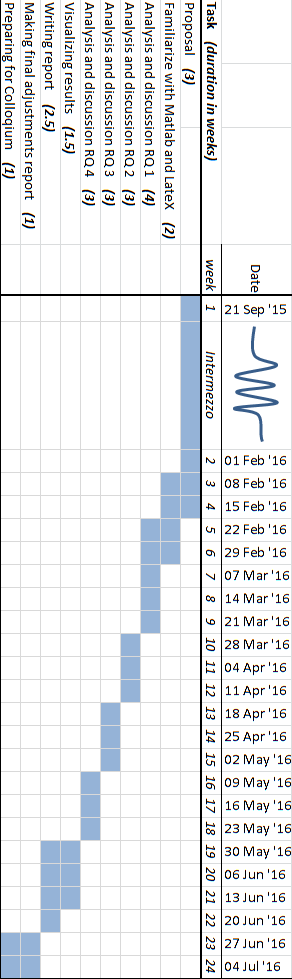
\includegraphics[height=7.5in]{figures/Planning.png}
	\caption[Optional caption]{Gantt chart of this study, indicating what I plan to be working on for each week. The planning also contains 'Intermezzo', which is the period where I could hardly work on my research due to health issues.}
	\label{fig:planning}
\end{figure}


\newpage

\printbibliography

%%%%%%%%%%%%%%%%
%% Backmatter %%
%%%%%%%%%%%%%%%%


\newpage
\section*{Appendices} % Appendices


\subsection*{Appendix A - satellite and imager properties}\label{appendix:A}
Tables with properties of the SEVIRI imager and the MSGCPP product of the KNMI.

 \begin{table}[H]
	\centering
	\label{tab:seviriproperties}
	\caption{Spectral channel characteristics of the SEVIRI in terms of central, minimum and maximum wavelength of the channels and the main application areas of each channel.}
	\begin{tabular}{@p{2cm}^p{2cm}^p{1.5cm}^p{1.5cm}^p{1.5cm}^p{5cm}}
		\hline \rowstyle{\bfseries}Channel No.	& Spectral Band ($\mu m$) & \multicolumn{3}{c}{\rowstyle{\bfseries}Characteristics of  Spectral Band ($\mu m$)} & Main observational applications \\ \hline
		 & & cen & min &	max	& \\ \hline
		1 &	VIS0.6 &	0.635	& 0.56 & 0.71	& Surface, clouds, wind fields \\
		2 &	VIS0.8 &	0.81 &	0.74 &	0.88 &	Surface, clouds, wind fields \\
		3 &	NIR1.6 &	1.64 &	1.50 &	1.78 &	Surface, cloud phase \\
		4 &	IR3.9 &	3.90 &	3.48 &	4.36 &	Surface, clouds, wind fields\\
		5 &	WV6.2 &	6.25 &	5.35 &	7.15 &	Water vapor, high level clouds, atmospheric instability\\
		6 &	WV7.3 &	7.35 &	6.85 &	7.85 &	Water vapor, atmospheric instability\\
		7 &	IR8.7 &	8.70 &	8.30 &	9.1 &	Surface, clouds, atmospheric instability\\
		8 &	IR9.7 &	9.66 &	9.38 &	9.94 &	Ozone\\
		9 &	IR10.8 &	10.80 &	9.80 &	11.80 &	Surface, clouds, wind fields, atmospheric instability\\
		10 & IR12.0 & 12.00 &	11.00 &	13.00 &	Surface, clouds, atmospheric instability\\
		11 & IR13.4 & 13.40 &	12.40 &	14.40 &	Cirrus cloud height, atmospheric instability\\
		12 & HRV & \multicolumn{3}{c}{Broadband (about 0.4 – 1.1 $\mu m$)} & Surface, clouds\\ \hline
	\end{tabular}
 \end{table}
 
  \begin{table}[H]
  	\begin{threeparttable}
	  	\small
	  	\centering
	  	\label{tab:msgcpp}
	  	\caption{List of MSG Cloud Physical Products and their reported validation accuracies.}
	  	\begin{tabular}{@p{2.2cm}^p{7cm}^p{2cm}^p{4.5cm}}
	  		\hline \rowstyle{\bfseries}ID	& Product & Unit & Accuracy\\ \hline
	  		\bfseries{CLDMASK} & Cloud Fraction & [-] & 0.1 \\ \hline
	  		\bfseries{CPH} & Cloud Thermodynamic Phase & [-] & 0.1 \\ \hline
	  		\bfseries{COT} & Cloud Optical Thickness & [-] & 15\% \\ \hline
	  		\bfseries{REFF} & Particle Size & [m] & - \\ \hline
	  		\bfseries{CTT} & Cloud Top Temperature & [K] & 5K \\ \hline
	  		\bfseries{CTH} & Cloud Top Height & [m] & - \\ \hline
	  		\bfseries{DCLD*} & Geometrical Depth & [m] & 250m \\ \hline
	  		\bfseries{DnDv*} & Droplet Number Concentration & [m-3] & - \\ \hline
	  		\bfseries{CWP**} & Condensed Water Path & [kg m-2] & 0.15x10-3 kg m-2 \\ \hline
	  		\bfseries{SDS} & Surface Downwelling Solar rad. & [W m-2] & 8 W m-2 \\ \hline
	  		\bfseries{SDS\textunderscore CS} & Clear-Sky Surface Downwelling Solar rad. & [W m-2] & 7 \\ \hline
	  		\bfseries{SDS\textunderscore DIFF} & Surface Downwelling Solar Diffuse rad. & [W m-2] & 7 \\ \hline
	  		\bfseries{SDS\textunderscore DIFF\textunderscore CS} & Clear-Sky Surface Downwelling Solar Diffuse rad. & [W m-2] & 11 \\ \hline
	  		\bfseries{PRECIP} & Rain Rate & [m s-1] & 2.8 x 10-7 m s-1 (=1 mm hr-1) \\ \hline
		\end{tabular}
		\begin{tablenotes}
			\item *) These products are only retrieved for liquid water clouds.
			\item **) Note, this is a combined product, The CWP for liquid water clouds represents the Liquid Water Path, CWP for ice clouds represents the Ice Water Path.
		\end{tablenotes}
	\end{threeparttable}
		
 \end{table}


		




\end{document}